\section{Introduction}

Curating learning assignments is a crucial step in practice-oriented education, especially when the goal is to help learners develop practical skills.
A well-orchestrated assignment turns abstract learning objectives into concrete learner actions: learners practice by working through meaningful project tasks, making design decisions, and producing artifacts that can be inspected and evaluated~\cite{blumenfeld1991motivating,barron1998doing}.
However, crafting such assignments is non-trivial and time-consuming for teachers, because it requires the joint design of tasks, supporting materials, scaffolding, and evaluation criteria.
This motivates the need to explore automated methods for designing learning assignments while preserving meaningful learner work.

As shown in Figure~\ref{fig:demo}, designing such assignments requires preparing resources for both learners and instructors.
For learners, project materials define the concrete working context, including starter files, task instructions, requirements, resources, and expected deliverables.
For instructors, instructional procedures specify how the assignment should be taught, supported, and evaluated, including learning objectives, scaffolding strategies, checkpoints, assessment criteria, and feedback mechanisms.
These two sides must be designed jointly: materials for learners determine what work learners can perform, while guidance for instructors determines what that work is meant to teach and how progress should be assessed.

\begin{figure}[t]
    \centering
    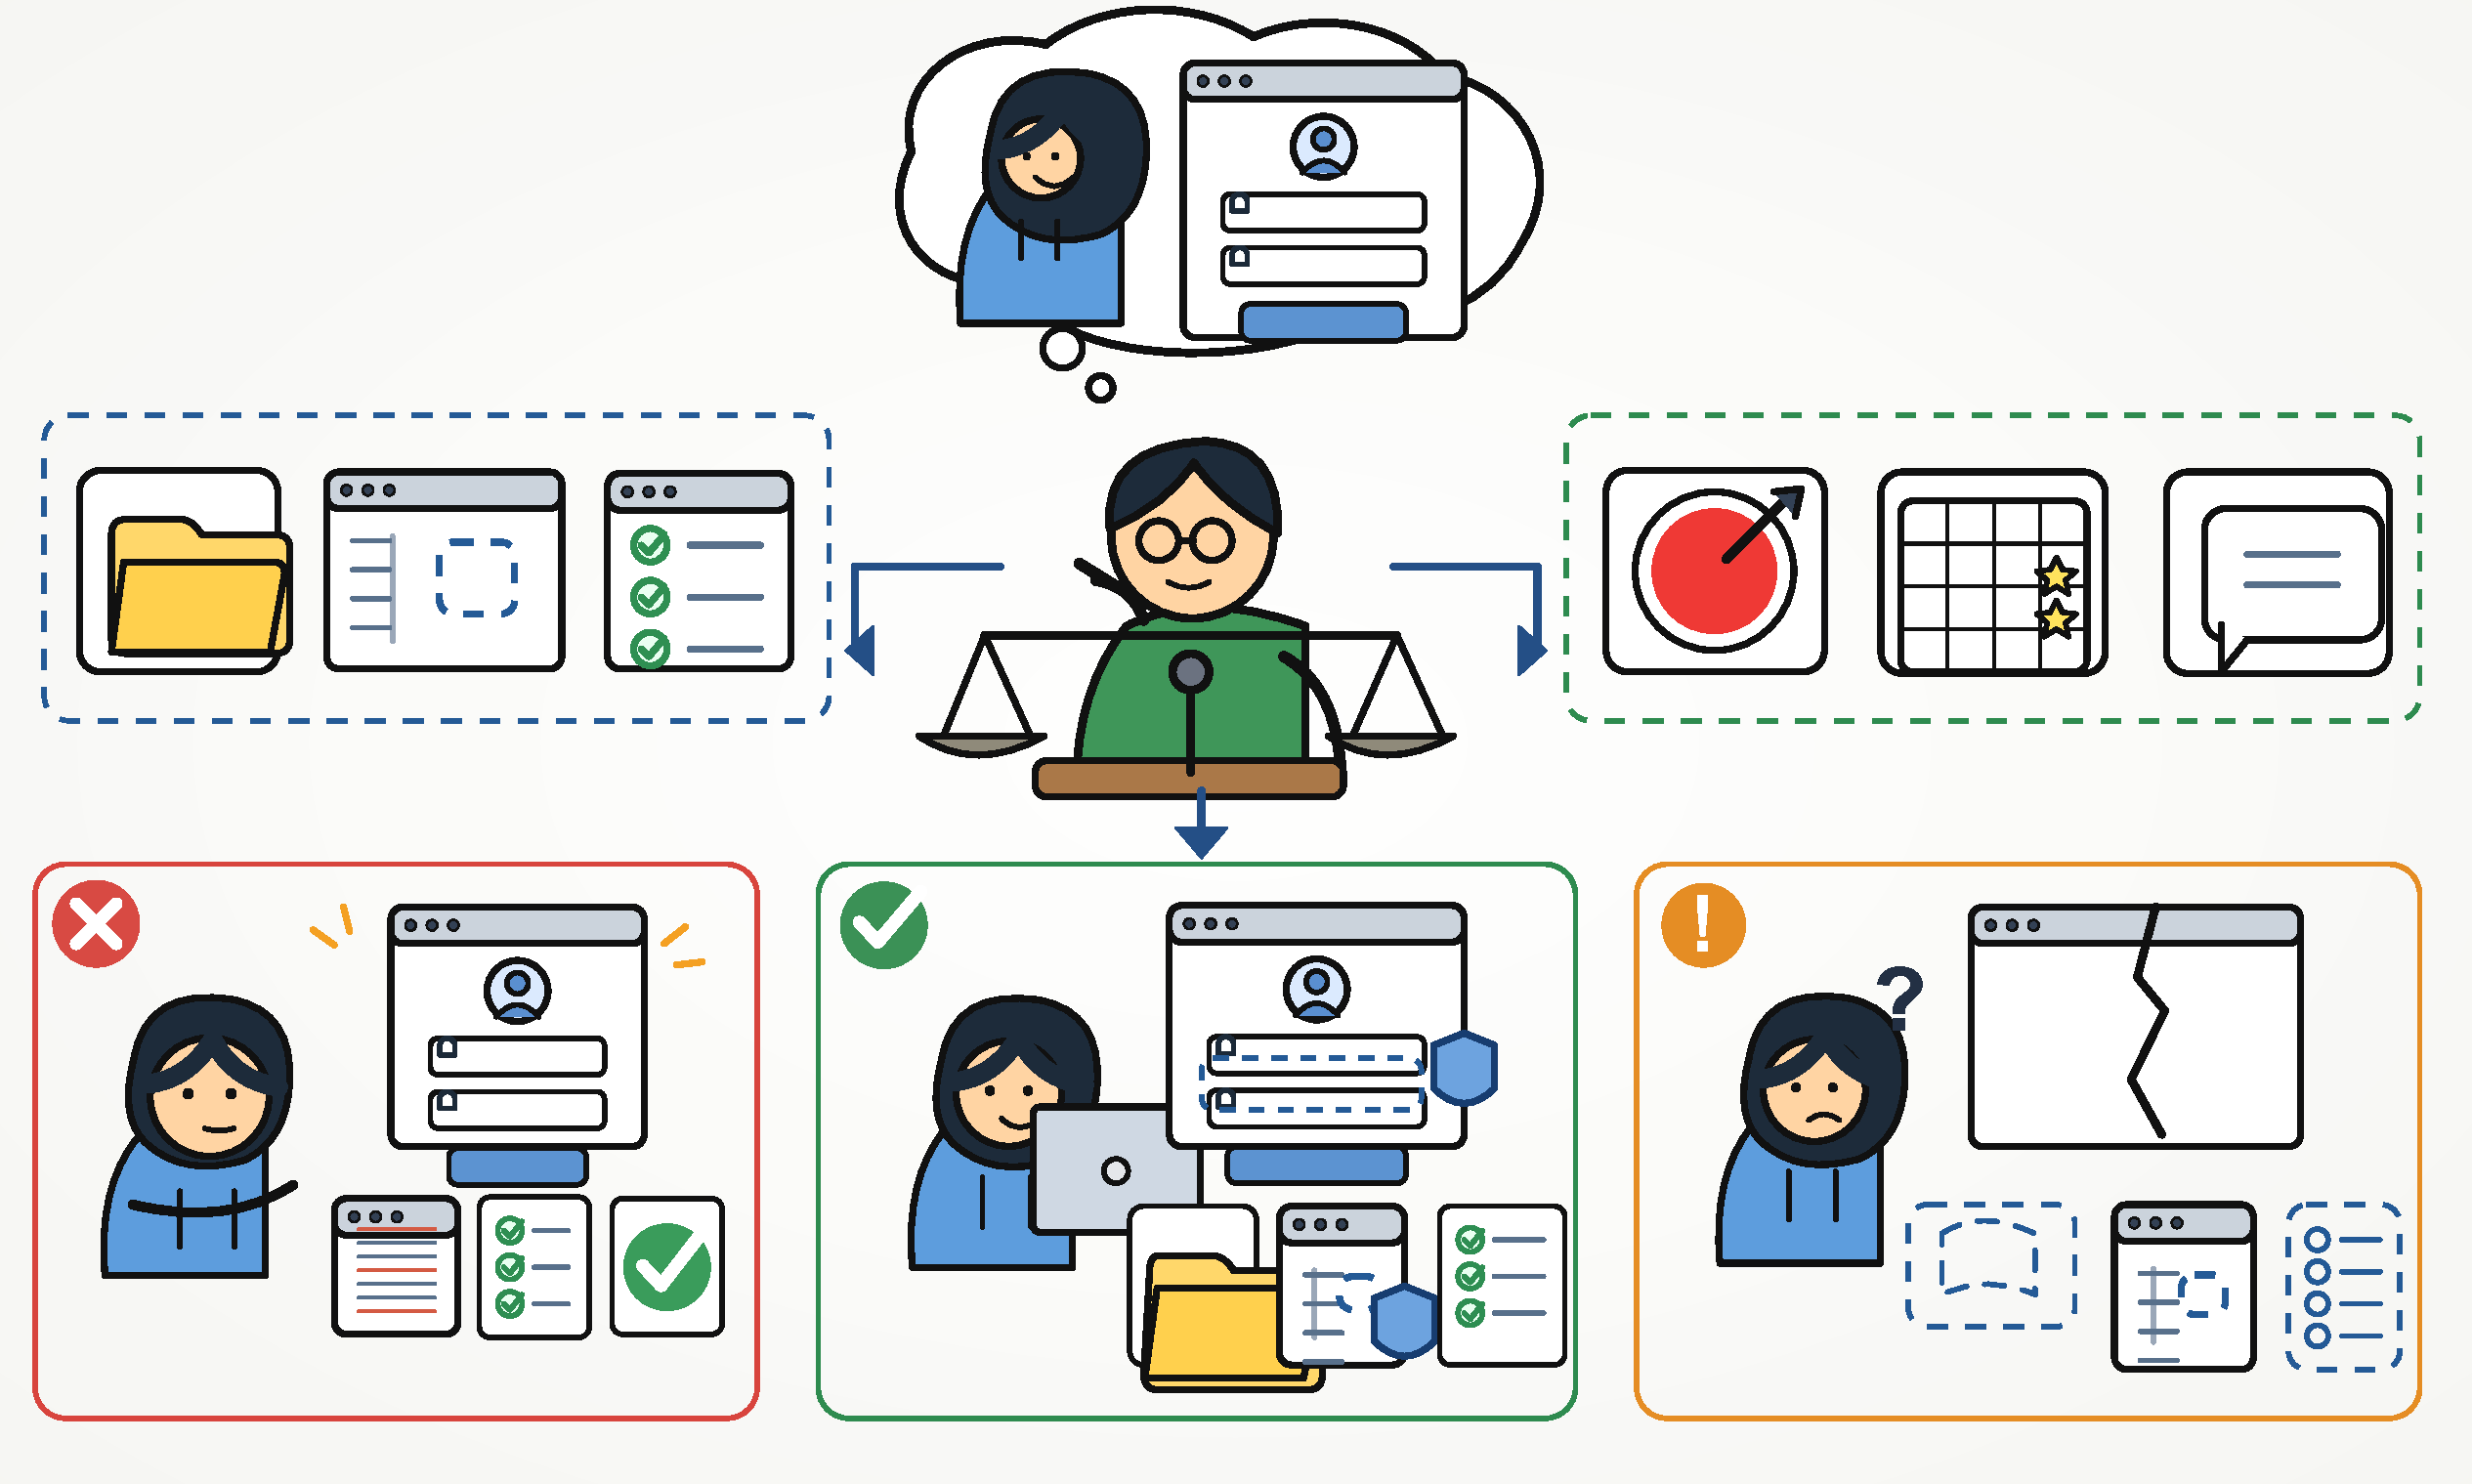
\includegraphics[width=\linewidth]{figures/demo-replica.pdf}
    \caption{Practice-assignment design requires coordinating learner-facing project materials with instructor-facing guidance so that the resulting assignment is executable while preserving meaningful learner-owned work.}
    \label{fig:demo}
\end{figure}

The difficulty is not only that these materials are numerous, but that they must remain coherent with one another.
The materials for learners must provide enough structure for students to make progress, while leaving open the parts of the task where learning should occur.
At the same time, the guidance for instructors must make clear why those parts are left open, how learners should be supported, and how their work should be assessed.
This makes assignment design both an engineering and a pedagogical problem: the system must decide what to build, what to scaffold, and what to leave for the learner.
These decisions interact: changing the project goal can change the required scaffolding, and changing the scaffolding can change what counts as meaningful learner work.


Existing LLM systems address parts of this engineering-pedagogical problem, but not the full assignment-design process.
Repository-level agents can generate and modify runnable code-bases~\cite{qian2023chatdev,hong2023metagpt,yang2024sweagent,wang2024openhands,zhang2024codeagent,shi2025autop2c}.
However, they are built to complete software artifacts, whereas a learning assignment must preserve selected work for the learner to perform.
In contrast, educational AI systems generate instructional content or support learning interactions, such as slides, question answering, textbooks, tutoring, scaffolding, and classroom simulation~\cite{zheng2025pptagent,zheng2026deeppresenter,shao2024storm,sharma2025pustakai,wang2024lessonplanner,zhang2024simclass,jang2026medtutor,cohn2026edf,deriyeva2026script,gao2024sinkt}.
These systems support instruction around a task, but typically do not generate a complete, aligned practice assignment.
Together, these gaps leave open a problem: how to turn a learner's goals into a complete, aligned practice assignment with meaningful learner work.


We propose \model, a framework for generating complete, aligned practice assignments from learner intent.
In this work, we realize these assignments as runnable training repositories tailored to individual learners.
\model first turns the learner's goals into an assignment plan that specifies the project materials, instructional procedures, target skills, scaffolding, and learner-owned work.
It then generates the corresponding repository components, including task instructions, starter files, scaffolds, tests, and validation behavior.
By coordinating materials for learners with guidance for instructors, \model aims to preserve meaningful learner work while scaling the creation of practice-oriented assignments.



\smallskip
\noindent In summary, our contributions are:
\begin{list}{$\bullet$}{%
    \setlength{\leftmargin}{1em}
    \setlength{\labelwidth}{0.5em}
    \setlength{\labelsep}{0.3em}
    \setlength{\itemsep}{0.2em}
    \setlength{\topsep}{0.2em}
    \setlength{\parsep}{0pt}
}
    \item We formulate practice-assignment generation as the task of transforming learner intent into complete, aligned assignments that coordinate project materials for learners, instructional guidance for instructors, and meaningful learner work.
    \item We introduce \model, a human-in-the-loop generation framework that coordinates project materials, instructional guidance, learner-aware scaffolding, repository construction, and validation to produce runnable training repositories with appropriate learner-owned work.
    \item We evaluate \model against direct generation baselines using both engineering and pedagogical criteria, showing improvements in repository validity, assignment alignment, and learner-work preservation.
\end{list}
